\documentclass[border=8pt]{standalone}
\usepackage{fontspec}
\setmainfont{TeX Gyre Heros}[Ligatures=TeXOff]
\XeTeXgenerateactualtext=1
\setsansfont{TeX Gyre Heros}
\usepackage{tikz}
\usetikzlibrary{arrows.meta,positioning,shapes.geometric,shapes.misc,shapes.symbols,fit,backgrounds,calc,chains}
\definecolor{ink}{HTML}{111827}
\definecolor{band}{HTML}{F3F4F6}
\definecolor{band2}{HTML}{E5E7EB}
\definecolor{accent}{HTML}{1D4ED8}
\definecolor{accentlight}{HTML}{DBEAFE}
\definecolor{warn}{HTML}{B91C1C}
\definecolor{warnlight}{HTML}{FEE2E2}
\definecolor{ok}{HTML}{047857}
\definecolor{oklight}{HTML}{D1FAE5}
\tikzset{
  >={Stealth[length=2.6mm]},
  box/.style={draw=ink, line width=0.6pt, rounded corners=9pt, fill=white, align=center,
              inner sep=4pt, font=\small},
  pill/.style={box, rounded corners=13pt},
  key/.style={box, fill=accentlight, draw=accent, line width=0.9pt},
  soft/.style={box, fill=band},
  dec/.style={draw=ink, line width=0.6pt, diamond, aspect=2.2, align=center, inner sep=1.5pt,
              font=\footnotesize, fill=white},
  arr/.style={->, draw=ink, line width=0.6pt},
  darr/.style={->, draw=ink, line width=0.6pt, dashed},
  lbl/.style={font=\footnotesize, fill=white, inner sep=1.5pt},
  layer/.style={draw=band2, fill=band, rounded corners=6pt},
  title/.style={font=\bfseries\small, align=left, anchor=west},
}
\begin{document}
\sffamily\hyphenpenalty=10000\exhyphenpenalty=10000

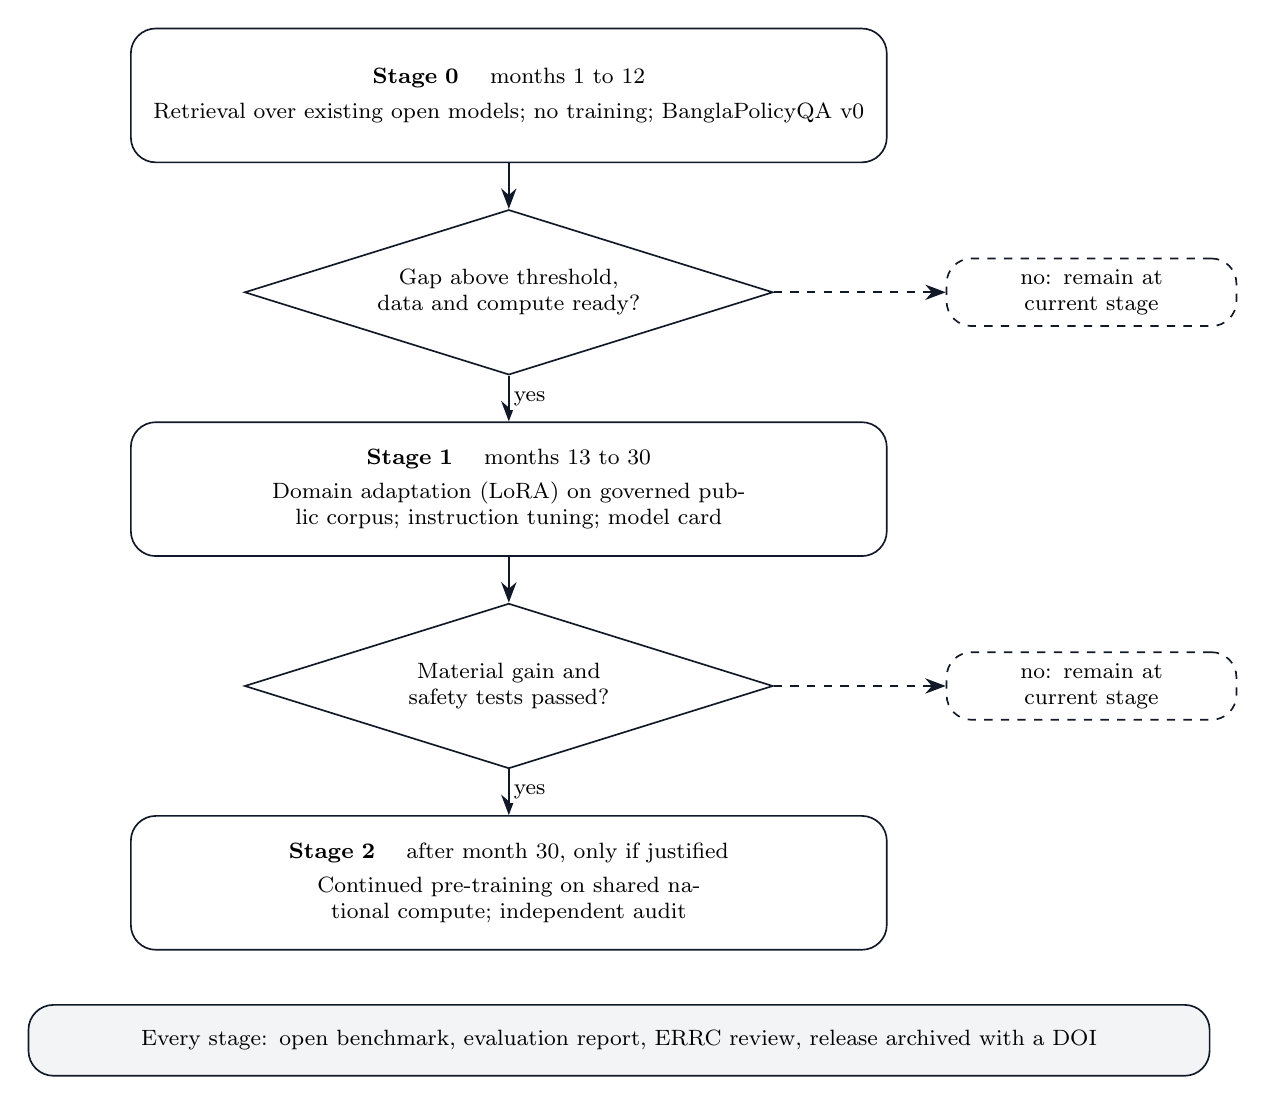
\begin{tikzpicture}
\tikzset{stage/.style={box, minimum width=96mm, minimum height=17mm, text width=92mm, font=\footnotesize},
         gate/.style={dec, aspect=3.2, text width=44mm, font=\footnotesize}}
\node[key, stage] (s0) at (0,0) {\textbf{Stage 0} \quad months 1 to 12\\[1mm]Retrieval over existing open models; no training; BanglaPolicyQA v0};
\node[gate] (g1) at (0,-25mm) {Gap above threshold, data and compute ready?};
\node[stage] (s1) at (0,-50mm) {\textbf{Stage 1} \quad months 13 to 30\\[1mm]Domain adaptation (LoRA) on governed public corpus; instruction tuning; model card};
\node[gate] (g2) at (0,-75mm) {Material gain and safety tests passed?};
\node[stage] (s2) at (0,-100mm) {\textbf{Stage 2} \quad after month 30, only if justified\\[1mm]Continued pre-training on shared national compute; independent audit};
\draw[arr] (s0) -- (g1);
\draw[arr] (g1) -- node[lbl, right]{yes} (s1);
\draw[arr] (s1) -- (g2);
\draw[arr] (g2) -- node[lbl, right]{yes} (s2);
\node[box, dashed, font=\footnotesize, text width=34mm] (st1) at (74mm,-25mm) {no: remain at current stage};
\node[box, dashed, font=\footnotesize, text width=34mm] (st2) at (74mm,-75mm) {no: remain at current stage};
\draw[darr] (g1) -- (st1); \draw[darr] (g2) -- (st2);
\node[soft, minimum width=150mm, text width=146mm, minimum height=9mm, font=\footnotesize] at (14mm,-120mm) {Every stage: open benchmark, evaluation report, ERRC review, release archived with a DOI};
\end{tikzpicture}
\end{document}
